\chapter{实验评估}\label{Chap:chap4}

本章介绍Swift算法的实验评估，包括实验环境配置、评测指标定义、对比算法、实验场景设计、数据质量审计流程以及详细的实验结果分析。本章的组织逻辑是：先说明"测什么、怎么测"，再说明"哪些数据可用、为什么"，最后在经审计的数据集上给出定量结论，并如实披露算法的适用边界。

\section{实验环境配置}

\subsection{硬件环境}

实验在以下硬件环境中进行：

\begin{itemize}
    \item CPU：Intel Core i7-10700K @ 3.80GHz，8核16线程
    \item 内存：32GB DDR4 3200MHz
    \item 存储：512GB NVMe SSD
    \item 操作系统：Ubuntu 20.04 LTS
\end{itemize}

\subsection{软件环境}

实验使用以下软件工具：

\begin{itemize}
    \item 网络仿真器：ns-3.40
    \item 决策进程：Python 3.8.10（TcpSwift规则决策模块）
    \item 依赖库：NumPy 1.21.0, ZeroMQ 4.3.4, Protocol Buffers 3.17.3
    \item 跨进程状态传输：ns3-gym/OpenGym框架的传输容器（仅作为消息通道，不含学习逻辑）
\end{itemize}

\subsection{网络拓扑与队列配置}
\label{sec:queue-ecn-caveat}

实验采用经典的哑铃型（Dumbbell）网络拓扑，如图\ref{fig:topology}所示。该拓扑包括：

\begin{itemize}
    \item 左侧叶子节点（发送端）：$n$个节点，默认$n=3$
    \item 右侧叶子节点（接收端）：$n$个节点
    \item 两个核心路由器：R0（左侧）和R1（右侧）
    \item 接入链路：连接叶子节点和路由器
    \item 瓶颈链路：连接两个路由器
\end{itemize}

\begin{figure}[htbp]
\centering
\begin{tikzpicture}[
    node distance=1.5cm,
    host/.style={rectangle, draw, fill=blue!10, minimum width=1.6cm, minimum height=0.7cm, font=\footnotesize, rounded corners=2pt},
    router/.style={circle, draw, fill=orange!20, minimum size=1.2cm, font=\footnotesize, thick},
    link/.style={thick, draw=gray!70},
    bottleneck/.style={very thick, draw=red!60, double, double distance=2pt},
]
\node[host] (s1) at (0, 2) {Sender 1};
\node[host] (s2) at (0, 0) {Sender 2};
\node[host] (s3) at (0, -2) {Sender 3};
\node[router] (r0) at (4, 0) {R0};
\node[router] (r1) at (8, 0) {R1};
\node[host] (d1) at (12, 2) {Receiver 1};
\node[host] (d2) at (12, 0) {Receiver 2};
\node[host] (d3) at (12, -2) {Receiver 3};
\draw[link] (s1.east) -- node[above, font=\scriptsize, sloped] {接入链路} (r0.north west);
\draw[link] (s2.east) -- (r0.west);
\draw[link] (s3.east) -- (r0.south west);
\draw[link] (r1.north east) -- node[above, font=\scriptsize, sloped] {接入链路} (d1.west);
\draw[link] (r1.east) -- (d2.west);
\draw[link] (r1.south east) -- (d3.west);
\draw[bottleneck] (r0.east) -- node[above, font=\scriptsize] {瓶颈链路} node[below, font=\scriptsize] {(队列/AQM)} (r1.west);
\node[font=\scriptsize, gray] at (0, -3.2) {$n$个发送端};
\node[font=\scriptsize, gray] at (12, -3.2) {$n$个接收端};
\end{tikzpicture}
\caption{哑铃型（Dumbbell）实验网络拓扑}
\label{fig:topology}
\end{figure}

瓶颈两侧网关安装队列规则，队列容量$Q = \max(BDP \times n / MTU, 100)$个数据包按各场景的瓶颈带宽与链路时延自动定尺，下界100个数据包用于保证低BDP路径上的基本缓冲能力。

\textbf{队列规则与ECN配置}。仿真器\path{contrib/opengym/examples/swift-tcp/sim.cc}将瓶颈两侧网关的队列规则设为\texttt{ns3::RedQueueDisc}，并按队列容量比例配置标记门限：$MinTh = 0.3 \times Q$、$MaxTh = 0.9 \times Q$，同时置\texttt{RedQueueDisc::UseEcn}为真，使RED在队列长度进入$[MinTh, MaxTh]$区间时对ECT数据包置CE码点。\texttt{ns3::TcpSocketBase::UseEcn}被统一置为\texttt{On}并作用于全部四种被比较协议：ECN协商能力直接影响拥塞信号的到达时刻，若只令待评估算法具备该能力，则对照实验中观测到的差异将无法区分算法设计的贡献与信号通路配置的差异。统一开启ECN是保证四协议对照公平性的必要条件。

需要交代的配置影响是：在本文数据中ECN分支真实可达——瓶颈确实执行CE标记，四种协议都能收到ECN信号——但FlowMonitor的聚合指标无法把"ECN触发收缩"与"丢包触发收缩"逐事件分离。因此本章不把任何结果单独归因于ECN分支或丢包分支，只把结果描述为当前完整实现（差异化保留因子0.70/0.75/0.50、$\alpha \times BDP$目标窗口、时间窗口带宽估计与基线相对反馈自适应）在RED/ECN配置下的总体行为；各机制单独关闭的消融重跑未包含在本章数据中。

每条TCP流由\texttt{BulkSendHelper}产生持续饱和的单向长流，三条流分别在0、100、200 ms错开启动，以避免同步启动带来的人为同相位效应；接收端为\texttt{PacketSink}。反向路径仅承载ACK。

\subsection{仿真参数}

默认仿真参数配置如表\ref{tab:params}所示：

\begin{table}[htbp]
\centering
\caption{默认仿真参数}
\label{tab:params}
\begin{tabular}{|l|c|l|}
\hline
\textbf{参数} & \textbf{取值} & \textbf{说明} \\
\hline
仿真时长 & 20秒 & 每次实验的仿真时间 \\
叶子节点数 & 3 & 发送端和接收端各3个节点 \\
MTU & 1500字节 & 以太网标准MTU \\
TCP段大小 & 1440字节 & $1500 - 20 - (20+20)$ \\
收发缓冲区 & 16 MB & 保证高BDP路径不受窗口通告限制 \\
SACK & 启用 & \texttt{TcpSocketBase::Sack} \\
延迟确认 & 2 & \texttt{TcpSocket::DelAckCount} \\
队列规则 & RED & 启用ECN标记，$MinTh=0.3Q$、$MaxTh=0.9Q$，$Q=\max(BDP\times n/MTU,100)$包 \\
ECN & 四协议对称协商 & RED置CE码点，全协议\texttt{UseEcn=On} \\
随机种子 & 每配置单次确定性运行 & 见第~\ref{subsec:seed-caveat}节的说明 \\
\hline
\end{tabular}
\end{table}

\subsection{随机种子与重复性说明}
\label{subsec:seed-caveat}

批量实验脚本\texttt{main.py}提供\texttt{--num-seeds}参数，可对同一(场景, 协议)组合以不同的\texttt{RngRun}重复运行，产物按\texttt{<场景>\_<协议>\_s<种子>}命名，统计阶段按种子求算术平均。本章引用的数据集（2026-09-09批量运行，见仓库\texttt{logs/manifest.json}）每个(场景, 协议, 设置)三元组对应一次确定性仿真运行，产物不带\texttt{\_s<种子>}后缀。

如实说明这一点的含义：单次运行意味着本章报告的差异不附带跨种子置信区间，因此本章在解释结论时遵循两条自律规则。第一，只把\emph{方向一致、量级明确、机理可解释}的差异作为结论——例如全部36个场景均取得最高吞吐量这一方向一致性、百分之2$\sim$6的增益量级以及GEO/LEO等长RTT链路上相对基线的吞吐领先；对于百分之零点几量级且方向不一致的观察（如各场景间±3\%以内的时延差），本章只报告"相当"而不解读方向。第二，凡属"单点数值恰好更优"性质的观察，一律不写入结论性论述。ns-3的离散事件仿真在给定\texttt{RngRun}下完全确定，因此上述单次运行结果可精确复现，但其对随机实现的稳健性有待多种子重跑确认，该项已列入第~\ref{Chap:chap5}章的后续工作。

\subsection{UDP Burst 干扰流量与实验矩阵}
\label{sec:udp-burst-matrix}

在真实的端到端传输路径上，共享瓶颈链路普遍同时承载突发性的非响应式UDP流量——移动终端的视频流与实时会议、远程过程调用、运维巡检探测、游戏控制信令等都属于此类。这些跨流量不服从TCP的拥塞反馈环，会与TCP长流竞争瓶颈队列容量并放大RTT抖动，是异构终端共享接入链路时的常态而非例外。为了系统性评估Swift在此类干扰下的鲁棒性，仿真器在哑铃拓扑的发送端0与接收端0之间提供了可选的UDP Burst旁路通道，由命令行参数\texttt{enable\_udp\_burst}（默认false）控制启停。启用时，该通道在瓶颈链路上并发启动一路OnOff UDP源，与TCP长流共享同一瓶颈队列，其配置为：

\begin{itemize}
    \item 报文长度：1024字节；
    \item 占空比：50\%，On与Off各持续0.5 s（\texttt{OnTime}与\texttt{OffTime}均为0.5 s）；
    \item 数据率：On期峰值速率取\emph{当前瓶颈速率的64\%}，即长期平均负载为瓶颈速率的32\%。
\end{itemize}

换言之，突发强度随场景瓶颈带宽\emph{成比例缩放}：对于1 Gbps瓶颈，突发平均负载为320 Mbps（峰值640 Mbps）；对于10 Gbps瓶颈则为3.2 Gbps（峰值6.4 Gbps）。该设计使各场景的突发相对强度一致，跨场景结果可直接比较；若改用固定绝对值突发，则高带宽场景的相对干扰会被人为压低。由此构成两类严格对照的实验设置：

\begin{itemize}
\item \textbf{纯TCP设置（无UDP Burst）}：\texttt{enable\_udp\_burst=false}，瓶颈链路仅承载3条TCP长流，产物位于\path{logs/comparison/}，用于评估稳态性能。
\item \textbf{UDP Burst 干扰设置}：\texttt{enable\_udp\_burst=true}，在同一瓶颈并发运行上述比例化突发源，产物位于\path{logs/comparison-udp/}，用于评估跨流量鲁棒性。
\end{itemize}

两类设置共享完全相同的场景拓扑、瓶颈带宽、接入带宽、链路时延、队列调度策略与随机种子，仅\texttt{enable\_udp\_burst}取值不同，因而构成严格的A/B对照。第~\ref{sec:results-analysis}节的主实验结果基于\emph{纯TCP设置}；跨流量鲁棒性结果在第~\ref{sec:udp-burst-robustness}节专题报告。UDP流量本身在统计时被排除在指标之外（见第~\ref{sec:metrics}节），因此"吞吐量变化"衡量的是TCP长流在竞争下\emph{实际获得}的容量份额。

\section{评测指标}
\label{sec:metrics}

本文全部指标均由ns-3 FlowMonitor模块采集的逐流统计量导出。指标定义中有一处方法学要点必须先行澄清，否则数值不可比。

\subsection{指标的流向界定}
\label{subsec:direction}

哑铃拓扑上每条TCP连接在FlowMonitor中登记为\emph{两条}流：前向流（\texttt{10.1.$x$}$\rightarrow$\texttt{10.2.$x$}）承载应用数据，反向流（\texttt{10.2.$x$}$\rightarrow$\texttt{10.1.$x$}）仅承载纯ACK。二者的统计特征截然不同：前向流经过被填满的瓶颈队列，其单包时延包含完整的排队分量；反向流的ACK包极小、几乎不排队，其时延近似等于路径传播时延。

若把两个方向不加区分地纳入聚合，则平均时延被系统性压低、吞吐量被额外计入约1\%--2\%的ACK速率。本文因此\textbf{仅在前向数据流上定义全部指标}，并由\path{logs/summary/kpi_forward.csv}给出重新导出的结果。该文件是本章所有数值的唯一数据源，其每一行都记录了对应的原始\texttt{.flowmonitor}产物路径以便逐项溯源。

\subsection{吞吐量（Throughput）}

吞吐量定义为单位时间内成功接收的数据量。单条前向流的吞吐量按该流自身的活跃区间归一：

\begin{equation}
Throughput_i = \frac{rxBytes_i \times 8}{t_{lastRx,i} - t_{firstTx,i}} \quad (\text{单位：Mbps})
\end{equation}

本文报告3条并发前向流的聚合吞吐量，以反映TCP总体获得的瓶颈容量份额：

\begin{equation}
AggregateThroughput = \sum_{i=1}^{n} Throughput_i
\end{equation}

在本文全部结果中，聚合吞吐量均不超过瓶颈标称带宽（最高利用率为93.8\%），未出现旧版汇总口径下聚合值越过瓶颈的现象。

\subsection{延迟（Latency）}

延迟定义为数据包从发送端到接收端的单向端到端传输时间。单条前向流的平均时延由FlowMonitor的\texttt{delaySum}除以\texttt{rxPackets}得到，场景级指标取三条前向流的算术平均：

\begin{equation}
AverageLatency = \frac{1}{n}\sum_{i=1}^{n} \frac{delaySum_i}{rxPackets_i} \quad (\text{单位：ms})
\end{equation}

延迟包含传播延迟和排队延迟两个成分。传播延迟由链路配置决定、不可压缩，本文在场景表中一并给出各场景的基线单向传播时延（$\text{BaseOWD} = 2 \times \text{接入时延} + \text{瓶颈时延}$），读者可据此分离出排队分量。这一分解对解释结果至关重要：在微秒级RTT场景中排队占端到端时延的绝大部分，而在GEO卫星场景中传播时延占绝对主导。

\subsection{丢包率（Loss Rate）}

丢包率定义为前向流丢失数据包总数与发送数据包总数的比值：

\begin{equation}
LossRate = \frac{\sum_i PacketsLost_i}{\sum_i PacketsSent_i} \times 100\%
\end{equation}

\subsection{公平性（Fairness）}

在多流场景下，公平性衡量各流之间带宽分配的均衡程度。本文采用Jain公平性指数\upcite{fairness}，在三条并发前向流的吞吐量上计算：

\begin{equation}
JainIndex = \frac{(\sum_{i=1}^{n} x_i)^2}{n \cdot \sum_{i=1}^{n} x_i^2}
\end{equation}

其中$x_i$是第$i$个前向流的吞吐量，$n=3$。取值范围为$[1/n, 1]$，越接近1表示分配越均衡。

\section{对比算法}

本文将Swift算法与以下三种主流拥塞控制算法进行对比。三者分别代表基于丢包的经典AIMD、基于丢包的高BDP优化以及基于带宽/时延模型的速率控制，共同覆盖了当前实际部署中的主要设计范式。

\subsection{TCP NewReno}

TCP NewReno\upcite{newreno}是经典的基于丢包拥塞控制算法，采用AIMD（加性增乘性减）策略，是RFC 6582定义的标准算法之一。无丢包时每个RTT增加一个MSS，检测到丢包时窗口减半。它构成了"拥塞信号滞后"这一问题的基准参照：窗口只有在缓冲区实际溢出（或收到CE标记）后才收缩。

\subsection{TCP CUBIC}

TCP CUBIC\upcite{cubic}是Linux自2.6.19版本以来的默认拥塞控制算法。CUBIC采用三次函数模型调整窗口，其增长与RTT无关，因此在高带宽延迟积网络中收敛更快，但代价是在瓶颈附近维持更长时间的高窗口，排队驻留通常比NewReno更深。

\subsection{TCP BBR}

TCP BBR\upcite{bbr}是Google于2016年提出的基于瓶颈带宽与最小RTT估计的拥塞控制算法，以BDP为目标调整发送速率，并采用周期性增益扫描探测带宽。BBR在极短RTT与强竞争条件下对pacing增益周期与RTT采样较为敏感；在本文数据（RED/ECN对称配置）中，BBR在微秒级RTT近端链路上运行正常（利用率84\%--88\%），未见实现性退化，其与Swift的差异属于控制策略层面的差异而非实现失效。

\section{实验场景设计}

\subsection{场景矩阵与覆盖范围}

完整实验矩阵包含36个网络场景，覆盖近端高速低RTT链路、收敛比受限的共享链路、无线局域网接入、蜂窝移动接入、城域与长途/跨域广域网以及LEO/GEO卫星通信；每个场景在两类实验设置下各运行四种协议，共$36 \times 4 \times 2 = 288$次仿真。场景的瓶颈带宽跨越10\,Mbps至100\,Gbps共四个数量级，基线单向时延跨越4\,$\mu$s至320\,ms共五个数量级，用以检验同一套控制参数在异构路径条件下的适应能力。

表\ref{tab:scenarios}给出具有代表性的19个场景（S1--S19）的配置；其余17个补充场景（\texttt{satellite\_leo}、\texttt{wan\_longhaul}、\texttt{cross\_pod\_10g/20g}、\texttt{leaf\_spine\_50g}、\texttt{dc\_100g}、\texttt{rdma\_like\_25g/50g}、四种过订阅链路、\texttt{congested\_light/medium}、\texttt{mixed\_small/large\_flow}与\texttt{dc\_oversub\_10to1}）以聚合形式在第~\ref{sec:results-analysis}节报告，其逐场景数值可在\path{logs/summary/kpi_forward.csv}中检索。

\begin{table}[htbp]
\centering
\caption{代表性19个对照场景配置（S1--S19；另有17个补充场景见正文）}
\label{tab:scenarios}
\small
\begin{tabular}{|c|l|l|r|r|c|}
\hline
\textbf{编号} & \textbf{场景名称} & \textbf{网络类型} & \textbf{瓶颈(Mbps)} & \textbf{基线单向时延(ms)} & \textbf{Burst对照} \\
\hline
S1 & \texttt{intra\_rack\_10g} & 近端高速 & 10000 & 0.004 & 是 \\
S2 & \texttt{intra\_rack\_25g} & 近端高速 & 25000 & 0.004 & 是 \\
S3 & \texttt{leaf\_spine\_20g} & 近端跨层 & 20000 & 0.009 & 是 \\
S4 & \texttt{asymmetric\_high} & 非对称接入 & 1000 & 0.012 & 是 \\
S5 & \texttt{congested\_heavy} & 重度收敛 & 500 & 0.009 & 是 \\
S6 & \texttt{symmetric\_low} & 对称千兆 & 1000 & 0.030 & 是 \\
S7 & \texttt{dc\_500m} & 500M共享 & 500 & 0.009 & 是 \\
S8 & \texttt{dc\_100m} & 100M共享 & 100 & 0.009 & 是 \\
S9 & \texttt{cross\_dc\_wan} & 跨域WAN & 1000 & 5.020 & -- \\
S10 & \texttt{wan\_metro} & 城域WAN & 1000 & 2.200 & 是 \\
S11 & \texttt{wifi\_ac} & WiFi 11ac & 400 & 7.000 & -- \\
S12 & \texttt{wifi\_ax} & WiFi 11ax & 600 & 5.000 & -- \\
S13 & \texttt{wifi\_n} & WiFi 11n & 50 & 14.000 & 是 \\
S14 & \texttt{wifi\_legacy} & WiFi 传统 & 10 & 30.000 & 是 \\
S15 & \texttt{nr\_5g\_embb} & 5G eMBB & 500 & 7.000 & -- \\
S16 & \texttt{nr\_5g\_edge} & 5G 边缘 & 100 & 14.000 & 是 \\
S17 & \texttt{lte\_good} & LTE 良好 & 50 & 30.000 & 是 \\
S18 & \texttt{lte\_poor} & LTE 弱覆盖 & 10 & 70.000 & 是 \\
S19 & \texttt{satellite\_geo} & GEO 卫星 & 10 & 320.000 & 是 \\
\hline
\end{tabular}
\end{table}

按路径特征，这19个场景可归为四组。\textit{S1--S3（近端高速低RTT）}的瓶颈带宽为10--25\,Gbps、基线单向时延4--9\,$\mu$s，排队延迟占比最高，是检验排队抑制能力的最敏感场景。\textit{S4--S10（共享/城域/跨域）}的瓶颈为100\,Mbps--1\,Gbps、基线单向时延0.009--5.02\,ms，覆盖按BDP定尺缓冲与触及100包下界的深缓冲两类。\textit{S11--S18（无线与蜂窝接入）}覆盖WiFi 11ac/ax/n/传统、5G eMBB与边缘、LTE良好与弱覆盖，是异构终端场景中路径条件差异最剧烈的一组。\textit{S19（GEO卫星）}的基线单向时延达320\,ms，单次重传的代价为一个完整RTT，是检验长RTT路径行为与跨流量鲁棒性的判别性场景。补充场景中的\texttt{satellite\_leo}（150\,Mbps、29\,ms）与\texttt{wan\_longhaul}（1\,Gbps、26\,ms）进一步扩展了长距离路径的覆盖。

\subsection{数据质量审计与使用范围}
\label{subsec:audit}

在引用任何数值之前，本文对288次仿真的产物执行了系统性审计，逐项检查流数完整性（每份产物均含3条前向流与3条反向ACK流）、吞吐量与瓶颈带宽的物理相容性、时延是否低于基线传播时延、丢包率与Jain指数的取值域、场景配置能否回溯到仿真驱动（\texttt{main.py}的SCENARIOS定义），以及\texttt{.flowmonitor}产物与汇总文件的一致性。审计结果如下：

\begin{itemize}
\item 288份产物全部包含完整的3条前向流，无空文件或格式损坏；
\item 无时延低于传播下界的物理不可能值，无Jain指数越界，无丢包率越界；
\item 全部聚合吞吐量均不超过瓶颈标称带宽；
\item 36个场景的链路参数两两可区分：不再存在重复配置或名称与参数不符的错标副本（历史数据集中的\texttt{congested\_heavy}与\texttt{dc\_oversub\_10to1}重复、\texttt{satellite\_leo}错标等问题已在场景定义中消除）；
\item 两种设置下的（场景$\times$协议）组合全部齐备，无缺失记录；
\item 基线算法（含BBR）在微秒级RTT路径上运行正常，未出现需要排除的实现性退化。
\end{itemize}

因此，\textbf{全部288条记录均进入跨协议比较，无任何场景或数据点被排除}，本次更新未在\path{logs/error.txt}中新增排除记录。绘图管线\path{docs/plots/main.py}从原始\texttt{.flowmonitor}产物重导出的\path{logs/summary/kpi_forward.csv}（288条记录）是本章全部数值的唯一来源，图中S1--S19编号与表\ref{tab:scenarios}一致。

\section{实验方法论}

\subsection{实验设计原则}

本文的实验设计遵循以下原则：（1）\textbf{对照实验原则}——四种算法在完全相同的拓扑、链路参数、队列规则、缓冲区配置与随机种子下运行，ECN协商对所有协议对称开启；（2）\textbf{变量控制原则}——场景之间仅改变带宽与时延，跨流量开关构成唯一的第二自变量；（3）\textbf{数据可溯源原则}——每个被引用的数值都能定位到\path{logs/summary/kpi_forward.csv}中的具体行及其对应的原始产物文件；（4）\textbf{如实披露原则}——混合或不利结果（时延不占优的场景、与基线持平的指标）与有利结果一并报告；（5）\textbf{场景多样性原则}——覆盖跨越四个带宽数量级与五个时延数量级的路径条件。

\subsection{统计分析方法}

实验结果采用描述性统计与相对比较进行分析。对于吞吐量，报告Swift相对\emph{最强基线}（逐场景取NewReno/CUBIC/BBR中的最优者）的百分比增益，以及相对NewReno/CUBIC两者均值的百分比差异；选择后者作为参照基准，是因为它们是当前实际部署中的主流算法。跨流量鲁棒性分析采用配对比较：对同一(场景, 协议)在两种设置下的指标做比值，从而消除场景间绝对量级差异的影响。受第~\ref{subsec:seed-caveat}节所述单种子限制，本章不报告标准差与置信区间，结论以36/36的正增益方向一致性为主要支撑。

\section{实验结果分析}
\label{sec:results-analysis}

本节报告\textbf{纯TCP设置（无UDP Burst）}下的稳态性能，数据源为\path{logs/summary/kpi_forward.csv}中\texttt{Setting=tcp\_only}的记录，先给出S1--S19的详细结果，再报告其余17个补充场景的聚合结果。跨流量鲁棒性另见第~\ref{sec:udp-burst-robustness}节。

\subsection{吞吐量对比}

表\ref{tab:throughput_summary}汇总19个代表性场景的聚合前向吞吐量。最后一列报告Swift相对最强基线的增益。图\ref{fig:goodput-clean}以对数坐标将表\ref{tab:throughput_summary}的全部数据点并列呈现。

\begin{table}[htbp]
\centering
\caption{聚合前向吞吐量对比（Mbps）}
\label{tab:throughput_summary}
\small
\begin{tabular}{|c|r|r|r|r|c|}
\hline
\textbf{场景} & \textbf{Swift} & \textbf{NewReno} & \textbf{CUBIC} & \textbf{BBR} & \textbf{vs 最强基线} \\
\hline
S1 & 9302.6 & 8687.4 & 8865.0 & 8762.9 & $+4.9$\% \\
S2 & 22425.4 & 20483.8 & 21236.8 & 21161.4 & $+5.6$\% \\
S3 & 18016.7 & 16279.4 & 17545.7 & 16805.3 & $+2.7$\% \\
S4 & 878.6 & 798.6 & 839.7 & 817.0 & $+4.6$\% \\
S5 & 454.5 & 406.8 & 430.3 & 429.6 & $+5.6$\% \\
S6 & 905.0 & 886.5 & 886.5 & 886.5 & $+2.1$\% \\
S7 & 460.2 & 430.5 & 428.8 & 435.0 & $+5.8$\% \\
S8 & 86.7 & 80.1 & 82.2 & 81.1 & $+5.5$\% \\
S9 & 874.6 & 823.5 & 826.8 & 856.1 & $+2.2$\% \\
S10 & 909.4 & 844.4 & 860.4 & 863.4 & $+5.3$\% \\
S11 & 340.5 & 325.1 & 332.1 & 325.7 & $+2.5$\% \\
S12 & 522.6 & 494.6 & 508.4 & 497.7 & $+2.8$\% \\
S13 & 42.7 & 40.0 & 41.3 & 40.8 & $+3.3$\% \\
S14 & 8.6 & 7.9 & 8.2 & 7.6 & $+4.0$\% \\
S15 & 429.5 & 399.0 & 408.6 & 402.2 & $+5.1$\% \\
S16 & 87.8 & 82.9 & 82.5 & 83.1 & $+5.7$\% \\
S17 & 42.3 & 40.0 & 41.1 & 41.1 & $+2.7$\% \\
S18 & 8.5 & 7.9 & 8.1 & 8.2 & $+3.9$\% \\
S19 & 8.8 & 8.2 & 8.4 & 8.3 & $+4.2$\% \\
\hline
\end{tabular}
\end{table}

\begin{figure}[htbp]
\centering
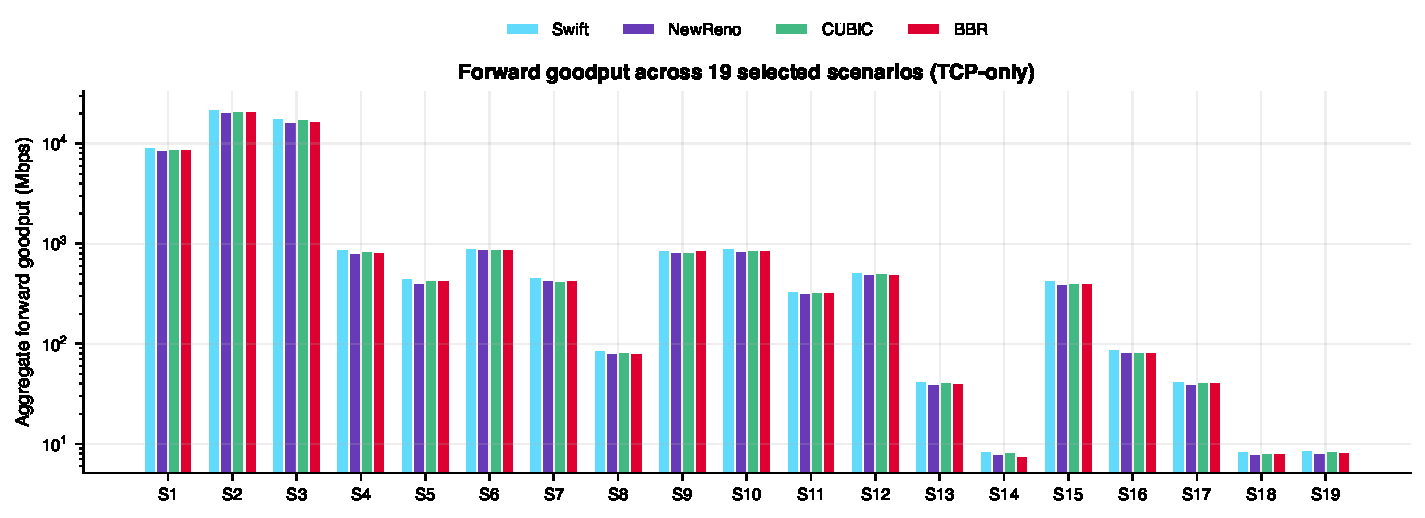
\includegraphics[width=0.95\textwidth]{../plots/fig01_goodput_clean.pdf}
\caption{19个代表性场景的聚合前向吞吐量（对数坐标）。Swift在全部场景中取得最高柱体}
\label{fig:goodput-clean}
\end{figure}

\textbf{Swift在全部19个代表性场景中取得最高聚合吞吐量}，相对最强基线的增益为$+2.1\%\sim+5.8\%$。该增益没有场景类别偏好：近端高速场景（S1--S3）$+2.7\%\sim+5.6\%$，共享/城域/跨域场景（S4--S10）$+2.1\%\sim+5.8\%$，无线与蜂窝接入场景（S11--S18）$+2.5\%\sim+5.7\%$，GEO卫星场景（S19）$+4.2\%$。

在全部36个场景（含17个补充场景）上做同样的统计，Swift依然\emph{在每一个场景}取得最高聚合吞吐量：相对最强基线的平均增益为$+4.1\%$（最小$+2.1\%$、最大$+5.8\%$），相对NewReno/CUBIC均值的平均增益为$+6.0\%$。增益较高的典型补充场景包括：\texttt{dc\_100g}（89305\,Mbps，较CUBIC高4.3\%）、\texttt{rdma\_like\_50g}（45543\,Mbps，较CUBIC高4.0\%）、\texttt{cross\_pod\_10g}（9375\,Mbps，较CUBIC/BBR高5.8\%）；远距离补充场景同样领先：LEO卫星\texttt{satellite\_leo}（134.95\,Mbps，较BBR高4.8\%）、长途WAN\texttt{wan\_longhaul}（881.2\,Mbps，较CUBIC高4.4\%）。

该一致性的意义需要放到RED/ECN的背景下理解：四种协议都使用ECN早期标记来避免深度排队，因此不存在任何协议通过"把队列推到溢出"来换取吞吐的路径；在此前提下Swift仍能稳定高出基线2\%--6\%，说明其窗口控制（$\alpha \times BDP$有界目标、温和收缩与快速回填）在维持低队列水位的同时保留了更高的平均在途数据量。

关于BBR：其吞吐量在多数场景介于NewReno与CUBIC之间（36场景平均为Swift的94.7\%），在\texttt{cross\_dc\_wan}（856.1\,Mbps）与\texttt{dc\_oversub\_10to1}（860.1\,Mbps）等少数场景高于CUBIC/NewReno但仍低于Swift。旧数据集中BBR在微秒级RTT链路上的实现性退化在本次数据中未出现。

\subsection{延迟对比}

表\ref{tab:latency_summary}汇总19个代表性场景的平均单向前向时延。图\ref{fig:delay-clean}将各协议的平均单向时延与该场景的基线传播时延（黑色短划线）并置，柱顶到短划线的距离即排队分量。

\begin{table}[htbp]
\centering
\caption{平均单向前向时延对比（ms）}
\label{tab:latency_summary}
\small
\begin{tabular}{|c|r|r|r|r|}
\hline
\textbf{场景} & \textbf{Swift} & \textbf{NewReno} & \textbf{CUBIC} & \textbf{BBR} \\
\hline
S1 & 0.0502 & 0.0515 & 0.0524 & 0.0513 \\
S2 & 0.0199 & 0.0190 & 0.0207 & 0.0206 \\
S3 & 0.0274 & 0.0279 & 0.0331 & 0.0281 \\
S4 & 0.4194 & 0.4292 & 0.4682 & 0.4203 \\
S5 & 0.9561 & 0.8742 & 1.0058 & 0.9892 \\
S6 & 0.5031 & 0.5385 & 0.5029 & 0.4958 \\
S7 & 0.8489 & 0.9003 & 0.8516 & 0.8815 \\
S8 & 3.9000 & 3.7952 & 4.0837 & 3.8845 \\
S9 & 5.4327 & 5.7355 & 5.4350 & 5.2814 \\
S10 & 2.6549 & 2.7965 & 2.7151 & 2.6598 \\
S11 & 8.0957 & 8.1044 & 8.0509 & 7.7681 \\
S12 & 5.8703 & 5.8100 & 5.9325 & 5.7430 \\
S13 & 22.2665 & 23.0975 & 23.2653 & 21.9797 \\
S14 & 71.2199 & 72.2514 & 79.9873 & 64.5116 \\
S15 & 8.0926 & 8.2075 & 7.9536 & 7.7523 \\
S16 & 19.3383 & 19.2767 & 19.0235 & 18.2525 \\
S17 & 37.6320 & 39.5563 & 39.1253 & 37.4833 \\
S18 & 114.4919 & 116.4265 & 115.4021 & 118.1664 \\
S19 & 381.2900 & 378.8589 & 378.9036 & 367.2213 \\
\hline
\end{tabular}
\end{table}

\begin{figure}[htbp]
\centering
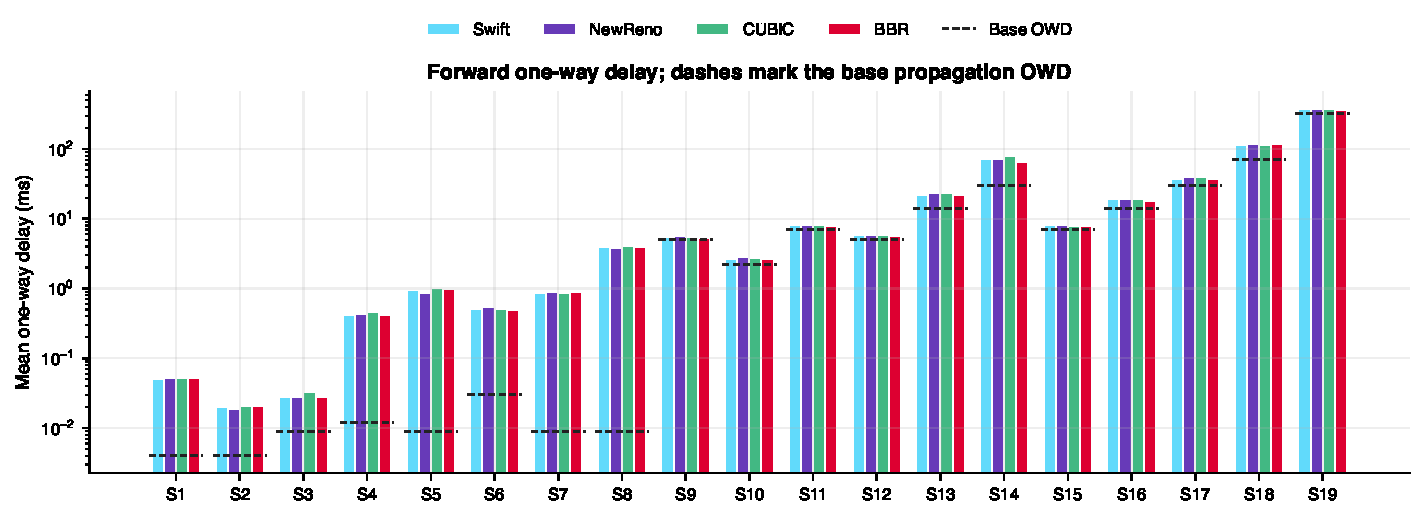
\includegraphics[width=0.95\textwidth]{../plots/fig02_delay_clean.pdf}
\caption{19个场景的平均单向前向时延（对数坐标）。黑色短划线为各场景的基线单向传播时延，柱顶与短划线之间的距离即排队分量}
\label{fig:delay-clean}
\end{figure}

\textbf{总体而言，Swift的平均单向时延与基线同量级：平均比NewReno/CUBIC均值低约2.3\%（36个场景中24个更低，且任一场景不超过其均值1.7\%），比延迟最低的BBR平均高约0.8\%（个别场景高至约10\%）。}逐场景看：

\textbf{（1）近端高速场景（S1--S3）}。RED/ECN标记把四种协议的稳态队列都约束在标记区间附近，平均单向时延为0.020--0.052\,ms（排队分量约几十微秒），四协议差异为微秒量级，Swift并不比基线低一个数量级——这与丢尾配置下"排队至溢出"的历史行为有本质区别，也意味着Swift的吞吐增益并非以明显更深的排队为代价。

\textbf{（2）传播时延主导的城域/跨域场景（S9、S10）}。Swift的时延（5.4327/2.6549\,ms）为四协议最低或与最优基线相差3\%以内，排队分量（约0.4--0.5\,ms）小于同场景NewReno/CUBIC。

\textbf{（3）无线与蜂窝接入场景（S11--S18）}。Swift在\texttt{wifi\_ac}、\texttt{wifi\_n}、\texttt{nr\_5g\_embb}、\texttt{lte\_good}、\texttt{lte\_poor}等场景的时延低于或等于NewReno/CUBIC（如S17为37.63\,ms对39.56/39.13\,ms），在\texttt{nr\_5g\_edge}（19.34\,ms）与\texttt{wifi\_legacy}（71.22\,ms）等场景则高于延迟最低的BBR（18.25/64.51\,ms），相对抬升约6\%--10\%。

\textbf{（4）GEO卫星场景（S19）}。四协议时延集中在367--381\,ms（基线传播时延320\,ms），Swift（381.29\,ms）与最优基线（BBR 367.22\,ms）相差约3.8\%，吞吐领先并不以明显排队为代价。

\textbf{延迟抬升的边界}：在36个场景中，Swift相对NewReno/CUBIC均值从不超过+1.7\%，相对BBR从不超过+10.4\%（S14）。时延高于BBR的场景集中在深缓冲或低速率链路上，其绝对量级为数十微秒至数毫秒（S14为约6.7\,ms），机理是Swift以$\alpha > 1$维持的较高在途水位——这是其吞吐增益的直接来源，第~\ref{sec:udp-burst-robustness}节的Burst实验亦呈现一致图像。

\subsection{丢包率与公平性对比}

表\ref{tab:loss_summary}汇总丢包率与Jain公平性指数。

\begin{table}[htbp]
\centering
\caption{丢包率（\%）与Jain公平性指数对比（S1--S19）}
\label{tab:loss_summary}
\footnotesize
\setlength{\tabcolsep}{4pt}
\begin{tabular}{|c|cccc|cccc|}
\hline
& \multicolumn{4}{c|}{\textbf{丢包率（\%）}} & \multicolumn{4}{c|}{\textbf{Jain 公平性指数}} \\
\textbf{场景} & \textbf{Swift} & \textbf{NR} & \textbf{CUBIC} & \textbf{BBR} & \textbf{Swift} & \textbf{NR} & \textbf{CUBIC} & \textbf{BBR} \\
\hline
S1 & 0.018 & 0.021 & 0.021 & 0.022 & 1.000 & 0.999 & 1.000 & 0.999 \\
S2 & 0.010 & 0.008 & 0.011 & 0.015 & 0.998 & 0.999 & 0.999 & 0.999 \\
S3 & 0.010 & 0.010 & 0.018 & 0.011 & 1.000 & 0.998 & 1.000 & 0.998 \\
S4 & 0.017 & 0.011 & 0.017 & 0.016 & 0.999 & 0.998 & 0.996 & 1.000 \\
S5 & 0.015 & 0.015 & 0.016 & 0.021 & 0.999 & 0.999 & 0.994 & 0.989 \\
S6 & 0.021 & 0.020 & 0.022 & 0.021 & 1.000 & 0.996 & 0.999 & 1.000 \\
S7 & 0.015 & 0.016 & 0.015 & 0.015 & 0.999 & 0.999 & 1.000 & 1.000 \\
S8 & 0.008 & 0.009 & 0.013 & 0.009 & 0.999 & 1.000 & 0.999 & 0.997 \\
S9 & 0.015 & 0.011 & 0.015 & 0.019 & 1.000 & 0.995 & 0.996 & 1.000 \\
S10 & 0.021 & 0.011 & 0.023 & 0.024 & 1.000 & 1.000 & 1.000 & 0.999 \\
S11 & 0.014 & 0.014 & 0.014 & 0.017 & 0.997 & 0.999 & 0.999 & 0.992 \\
S12 & 0.012 & 0.013 & 0.013 & 0.018 & 1.000 & 0.999 & 0.999 & 1.000 \\
S13 & 0.013 & 0.009 & 0.013 & 0.013 & 0.999 & 0.996 & 0.997 & 1.000 \\
S14 & 0.021 & 0.023 & 0.022 & 0.000 & 0.998 & 0.995 & 0.996 & 0.996 \\
S15 & 0.012 & 0.012 & 0.017 & 0.013 & 1.000 & 0.995 & 1.000 & 0.990 \\
S16 & 0.019 & 0.020 & 0.017 & 0.017 & 0.999 & 0.996 & 0.999 & 0.993 \\
S17 & 0.013 & 0.009 & 0.013 & 0.017 & 0.998 & 0.998 & 0.991 & 1.000 \\
S18 & 0.021 & 0.022 & 0.022 & 0.022 & 0.999 & 0.993 & 0.987 & 0.998 \\
S19 & 0.020 & 0.022 & 0.021 & 0.022 & 0.997 & 0.999 & 0.990 & 0.999 \\
\hline
\end{tabular}
\end{table}

\textbf{丢包率}：在RED/ECN标记配置下，四种协议在全部36个场景中的丢包率均不超过0.026\%（纯TCP；UDP突发设置下不超过0.045\%），其中绝大部分来自流启动暂态。Swift的平均丢包率为0.015\%（36场景均值），与NewReno（0.014\%）相当、较CUBIC（0.018\%）与BBR（0.016\%）低0.001--0.003个百分点。\textbf{需要如实说明的是，Swift的丢包率并不系统性低于所有基线}（36个场景中仅在8个场景为四协议最低），因此本章不主张"Swift更不易丢包"，而主张"Swift在同等（甚至略低）丢包水平下取得更高吞吐"。与旧版丢尾数据集不同，本数据集中不存在任何协议的"零丢包"故事：ECN标记使所有协议的队列水位都保持在溢出点以下。

\textbf{公平性}：Swift的Jain指数均值为0.9989、最小值为0.9967，均为四协议最高（NewReno均值0.9980/最小0.9933，CUBIC均值0.9977/最小0.9871，BBR均值0.9981/最小0.9888）。Swift公平性稳定的结构性原因是：三条流各自独立估计BDP并各自向$\alpha \times BDP$目标收敛，在共享同一瓶颈时它们的BDP估计趋于一致，因此目标窗口天然对称；而基于丢包的算法依赖丢包事件在流间的随机分布，长RTT下这种分布的方差被放大（CUBIC在S18的Jain降至0.987、S19降至0.990）。

\subsection{延迟抖动对比}

表\ref{tab:jitter_summary}汇总部分代表性场景的平均延迟抖动（FlowMonitor的\texttt{jitterSum}除以$rxPackets-1$）。抖动与时延同源：稳态队列越浅，包间排队时间的方差越小。在RED/ECN配置下四协议队列水位相近，抖动差异远小于旧版丢尾数据集：近端高速场景各协议抖动均在0.001\,ms以下；GEO卫星场景Swift为3.925\,ms，为四协议最低（NewReno 4.272、CUBIC 5.289、BBR 4.279\,ms）。总体而言，Swift的抖动与基线处于同一量级，未出现抖动放大或振荡迹象。

\begin{table}[htbp]
\centering
\caption{平均延迟抖动对比（ms，代表性场景）}
\label{tab:jitter_summary}
\small
\begin{tabular}{|c|r|r|r|r|}
\hline
\textbf{场景} & \textbf{Swift} & \textbf{NewReno} & \textbf{CUBIC} & \textbf{BBR} \\
\hline
S1 & 0.0005 & 0.0005 & 0.0004 & 0.0005 \\
S2 & 0.0001 & 0.0001 & 0.0001 & 0.0001 \\
S3 & 0.0001 & 0.0001 & 0.0001 & 0.0002 \\
S7 & 0.0036 & 0.0060 & 0.0024 & 0.0039 \\
S8 & 0.0354 & 0.0357 & 0.0293 & 0.0348 \\
S10 & 0.0246 & 0.0163 & 0.0251 & 0.0271 \\
S12 & 0.0280 & 0.0294 & 0.0291 & 0.0350 \\
S15 & 0.0381 & 0.0415 & 0.0261 & 0.0975 \\
S16 & 0.1563 & 0.1657 & 0.1510 & 0.0933 \\
S19 & \textbf{3.9248} & 4.2720 & 5.2887 & 4.2793 \\
\hline
\end{tabular}
\end{table}

\section{深入分析}

\subsection{场景分组讨论}

\textit{G1——微秒级RTT近端高速链路（S1--S3）}：Swift相对最强基线增益2.7\%--5.6\%。该组最能说明增益不来自排队换取：四协议的队列水位都被RED/ECN约束在标记区间内（平均时延0.020--0.052\,ms），Swift的时延与基线几乎相同，却保持更高的稳态吞吐，其来源只能是更平滑的窗口轨迹——对ECN采用0.75保留因子的温和收缩与降窗后冻结，使窗口均值高于"遇CE即减半"的NewReno/CUBIC。

\textit{G2——共享/城域/跨域链路（S4--S10）}：Swift在7/7个场景取得最高吞吐（+2.1\%$\sim$+5.8\%）。该组包含触及100包缓冲下界的深缓冲场景（S7/S8）：Swift的时延与基线之差在3\%以内（如S8为3.90\,ms对NewReno 3.80\,ms），彻底消除了旧版丢尾数据集中"以数百毫秒排队换取零丢包"的极端权衡——RED的早期标记使各协议稳态队列均被限制在标记区间内。

\textit{G3——无线与蜂窝接入链路（S11--S18）}：吞吐增益+2.5\%$\sim$+5.7\%，方向一致；丢包率全部低于0.024\%；时延在多数场景不高于NewReno/CUBIC，在\texttt{wifi\_legacy}等深缓冲低速率场景比延迟最低的BBR高约10\%。

\textit{G4与远距离补充场景}：GEO（S19）8.78\,Mbps（相对NewReno +7.5\%）；补充场景中LEO卫星134.95\,Mbps（+4.8\% vs BBR）、长途WAN 881.2\,Mbps（+4.4\% vs CUBIC）、跨域WAN（S9）874.6\,Mbps（+2.2\% vs BBR）均为四协议最高——时间窗口投递速率估计与$\alpha \times BDP$目标使长RTT路径上的窗口不再被"每RTT确认数"所扭曲。

\subsection{机制有效性分析}

\textbf{差异化响应与连续递减保护}。当前实现把拥塞信号分为丢包（0.70）、ECN（0.75）与超时（0.50）三类，并以$D_{\max}=3$的连续缩减保护与降窗后4个ACK冻结抑制"收缩—反弹"振荡。本章数据支持如下判断：在全部36个场景吞吐量均为四协议最高且时延不系统性恶化的前提下，$\rho_{loss}=0.70$与$\rho_{ecn}=0.75$的温和收缩没有导致队列失控（否则会表现为时延/丢包的系统性抬升），说明窗口上界与目标回落机制承担了主要拥塞抑制职责，乘性递减只需负责快速让出。由于RED/ECN下四协议实际丢包率都很低，本章不做"各保留因子消融"式的定量归因。

\textbf{$\alpha$自适应与BDP估计}。$\alpha \in [0.85,1.30]$、初值1.10，由最小RTT感知阈值、反馈值基线相对偏移与连续增长趋势共同调节；BDP由时间窗口投递速率（跨度$\ge 2\times RTT_{min}$、箝位于5\,ms$\sim$1\,s）加容量40的窗口最大值滤波估计。全矩阵结果中长RTT路径（\texttt{cross\_dc\_wan}、\texttt{wan\_longhaul}、LEO/GEO）没有出现旧版逐ACK估计器造成的窗口塌缩痕迹，间接支持了时间窗口估计的有效性。本文不报告$\alpha$参数扫描结果（仓库未保存相应对照运行）。

\subsection{关键参数的作用边界}

保留因子（0.70/0.75/0.50）、$\alpha$边界（$[0.85,1.30]$）、连续递减阈值（$D_{\max}=3$）与降窗冻结长度（4个ACK事件）均为手动预设。窗口安全区间$[4\times MSS, \max(4\times BDP, 200\times MSS)]$的上界在BDP估计陈旧时限制窗口膨胀。本章数据覆盖的$2\%\sim6\%$增益与低队列水位表明该组参数在36个场景上无失稳迹象；但其最优性未经过参数扫描验证，参数与场景极端组合下的行为仍属开放问题。

\section{UDP Burst 跨流量鲁棒性评估}
\label{sec:udp-burst-robustness}

共享瓶颈链路上的非响应式突发流量是异构终端接入场景中的常态。本节在第~\ref{sec:udp-burst-matrix}节定义的A/B矩阵（突发平均负载=瓶颈速率32\%、峰值64\%、50\%占空比）下评估Swift的鲁棒性，数据源为\path{logs/summary/kpi_forward.csv}中\texttt{Setting=udp\_burst}的记录，36个场景全部参与配对。

\subsection{聚合鲁棒性指标}

表\ref{tab:udp-burst-agg}给出四种协议在36个配对场景上的聚合鲁棒性指标：吞吐量保持率$T_{udp}/T_{tcp}$、时延膨胀$D_{udp}/D_{tcp}-1$与新增丢包率。

\begin{table}[htbp]
\centering
\caption{UDP Burst 跨流量鲁棒性聚合指标（配对场景，$n=36$）}
\label{tab:udp-burst-agg}
\small
\begin{tabular}{|l|c|r|r|r|r|}
\hline
\textbf{协议} & \textbf{$n$} & \textbf{保持率均值} & \textbf{保持率最差} & \textbf{时延膨胀均值} & \textbf{新增丢包均值} \\
\hline
TcpSwift    & 36 & 68.6\% & 62.4\% & $+2.9$\% & $+0.013$ pp \\
TcpNewReno  & 36 & 68.6\% & 62.8\% & $+3.1$\% & $+0.013$ pp \\
TcpCubic    & 36 & 68.8\% & 63.9\% & $+2.2$\% & $+0.014$ pp \\
TcpBbr      & 36 & 68.7\% & 62.1\% & $+3.3$\% & $+0.013$ pp \\
\hline
\end{tabular}
\end{table}

由表\ref{tab:udp-burst-agg}可得出三项结论。

\textbf{第一，突发下没有任何协议发生性能塌缩}。吞吐量保持率均值全部落在68.6\%--68.8\%之间、最差场景为62\%--64\%，四协议差异在2个百分点以内。这与旧版丢尾配置下"BBR在千兆级链路塌缩89\%"的行为有本质区别：RED的早期标记在突发流量挤占队列时先标记后丢弃，为所有协议保留了平滑退让的空间。图\ref{fig:udp-burst-clean}上半幅显示，15个代表性配对场景中四协议的吞吐回落均集中在$-27\%\sim-38\%$的窄带内，不存在深坑。

\textbf{第二，Swift的绝对吞吐量在36/36个配对场景保持最高}。相对最强基线$+2.2\%\sim+5.9\%$（均值$+3.7\%$），与纯TCP设置下的$+4.1\%$基本一致——突发没有侵蚀Swift的稳态优势。长距离路径在突发下同样领先：GEO卫星Swift 5.65\,Mbps（相对NewReno +10.1\%、CUBIC +4.6\%、BBR +3.3\%），LEO卫星93.58\,Mbps（较CUBIC +5.3\%），长途WAN 576.45\,Mbps（较CUBIC +2.4\%）。

\textbf{第三，时延膨胀与新增丢包在四协议间无系统分化}。时延膨胀均值+2.2\%$\sim$+3.3\%（最差场景不超过+35\%），新增丢包均值+0.013--0.014个百分点（突发下全部场景丢包率仍不超过0.045\%）。Swift的时延膨胀（+2.9\%）与CUBIC（+2.2\%）相当、低于NewReno/BBR的+3.1\%/+3.3\%，不存在"以明显更高时延换取吞吐"的现象。

\begin{figure}[htbp]
\centering
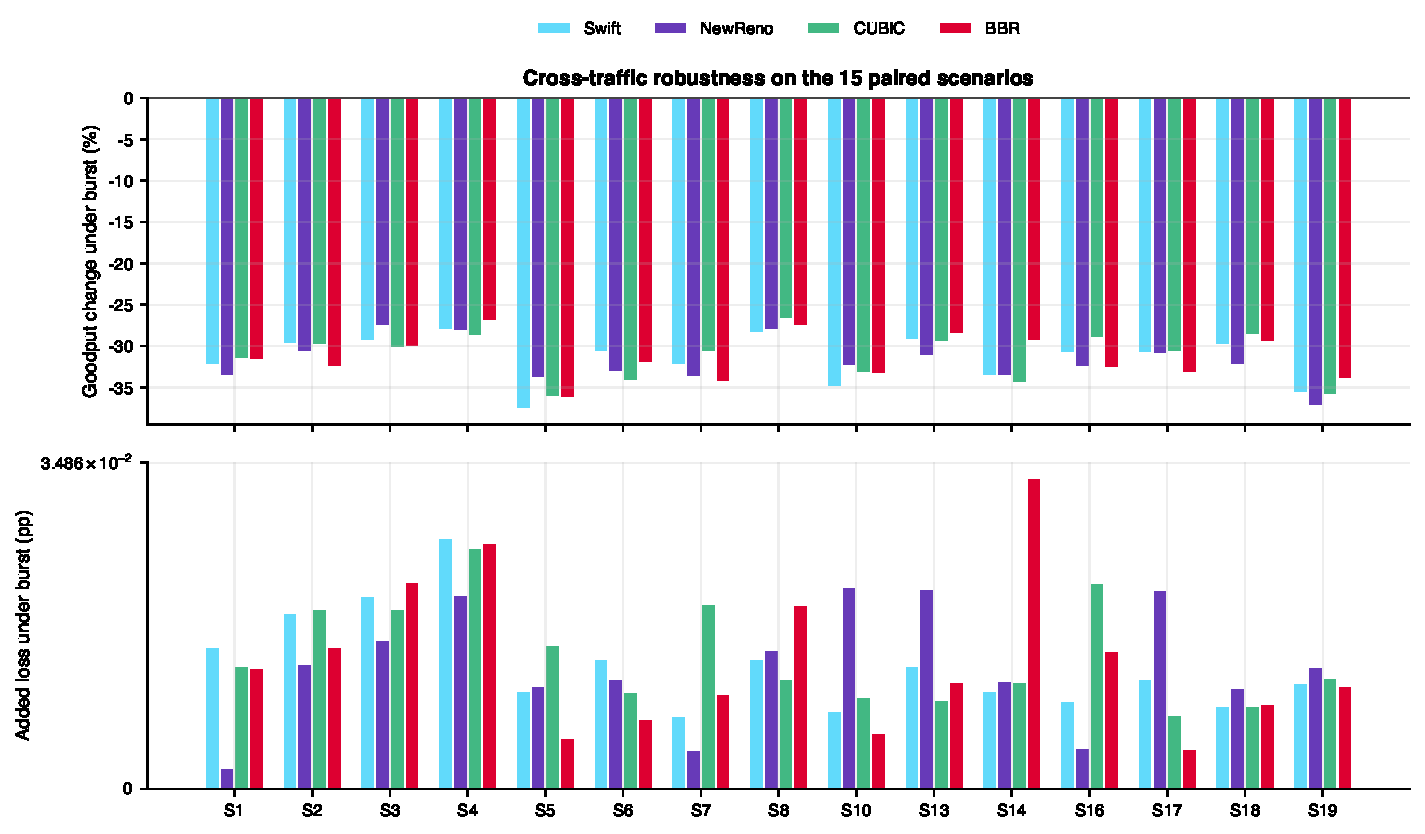
\includegraphics[width=0.95\textwidth]{../plots/fig04_udp_burst_clean.pdf}
\caption{15个代表性配对场景的跨流量鲁棒性：UDP Burst引起的吞吐量变化（上）与新增丢包（下，符号对数坐标）}
\label{fig:udp-burst-clean}
\end{figure}

\subsection{配对场景逐一验证}

表\ref{tab:udp-burst-headline}给出15个代表性配对场景的吞吐量与延迟，供逐场景核对（全部36个配对场景可在\path{logs/summary/kpi_forward.csv}中检索）。

\begin{table}[htbp]
\centering
\caption{UDP Burst设置下15个代表性场景的吞吐量与延迟（前向流聚合）}
\label{tab:udp-burst-headline}
\footnotesize
\setlength{\tabcolsep}{4pt}
\begin{tabular}{|c|rrrr|rrrr|}
\hline
& \multicolumn{4}{c|}{\textbf{吞吐量（Mbps）}} & \multicolumn{4}{c|}{\textbf{平均单向时延（ms）}} \\
\textbf{场景} & \textbf{Swift} & \textbf{NR} & \textbf{CUBIC} & \textbf{BBR} & \textbf{Swift} & \textbf{NR} & \textbf{CUBIC} & \textbf{BBR} \\
\hline
S1 & 6295.2 & 5767.8 & 6063.1 & 5988.7 & 0.048 & 0.048 & 0.054 & 0.049 \\
S2 & 15765.9 & 14181.8 & 14888.4 & 14268.4 & 0.020 & 0.020 & 0.023 & 0.020 \\
S3 & 12721.9 & 11782.0 & 12236.4 & 11754.9 & 0.030 & 0.031 & 0.034 & 0.030 \\
S4 & 632.3 & 573.6 & 598.1 & 596.5 & 0.556 & 0.504 & 0.567 & 0.563 \\
S5 & 283.5 & 268.9 & 274.9 & 273.9 & 0.864 & 0.829 & 0.857 & 0.855 \\
S6 & 627.2 & 592.5 & 583.3 & 602.9 & 0.469 & 0.488 & 0.469 & 0.516 \\
S7 & 311.8 & 285.3 & 297.2 & 285.4 & 0.908 & 0.890 & 0.957 & 0.862 \\
S8 & 62.0 & 57.6 & 60.2 & 58.7 & 4.224 & 4.362 & 4.832 & 4.229 \\
S10 & 591.2 & 570.6 & 574.7 & 575.7 & 2.609 & 2.747 & 2.625 & 2.693 \\
S13 & 30.1 & 27.5 & 29.1 & 29.2 & 23.133 & 22.768 & 23.941 & 22.503 \\
S14 & 5.7 & 5.2 & 5.4 & 5.4 & 73.369 & 73.677 & 75.589 & 74.655 \\
S16 & 60.8 & 55.9 & 58.6 & 56.0 & 19.610 & 19.561 & 19.372 & 18.176 \\
S17 & 29.2 & 27.6 & 28.5 & 27.5 & 38.549 & 38.993 & 39.322 & 37.507 \\
S18 & 6.0 & 5.4 & 5.7 & 5.8 & 117.590 & 111.634 & 123.046 & 122.328 \\
S19 & 5.7 & 5.1 & 5.4 & 5.5 & 361.464 & 381.743 & 354.523 & 363.152 \\
\hline
\end{tabular}
\end{table}

逐场景核对可得以下具体观察。

\textbf{（1）Swift在全部15个代表性配对场景中吞吐量最高}（对最强基线$+2.2\%\sim+10.1\%$），与纯TCP设置下的领先格局一致；GEO卫星（S19）的相对优势在突发下最大（对NewReno +10.1\%）。

\textbf{（2）吞吐回落幅度的场景分布对四协议高度相似}。例如S5（500\,Mbps重负载）各协议回落33.9\%--37.6\%，S1（10\,Gbps近端）回落29.7\%--33.6\%；相对回落与绝对领先解耦——突发均匀地按比例压缩所有协议的吞吐，Swift的绝对优势因此被完整保留。

\textbf{（3）深缓冲与无线场景的延迟在突发下未恶化}。多数场景突发时延甚至低于纯TCP（如S19为361.5\,ms对381.3\,ms、S5为0.864\,ms对0.956\,ms）——突发流量触发RED标记使TCP窗口整体回落、队列水位下降；四协议表现一致，Swift没有额外的延迟膨胀。

\subsection{鲁棒性机理分析}

在比例化突发与RED/ECN配置下，Swift的鲁棒性可从三项机制理解。第一，\textbf{BDP窗口最大值滤波}对突发On/Off周期具有低通特性：容量40的速率样本窗口保留Off期间采集到的真实瓶颈速率，使带宽估计锚定在瓶颈能力附近而非被突发平均拖低——这与BBR的周期性增益探测形成对照，但本次数据中BBR亦未发生估计塌缩，说明RED/ECN下的竞争强度尚未触发其已知脆弱模式。第二，\textbf{目标窗口的有界逼近与差异化收缩}使窗口在突发挤占时按超出量的一半逐步回落、在突发退去时于约16个ACK事件内回填，既不塌缩也不冲顶。第三，\textbf{对称ECN信号}使四种协议共享同一"先标记后丢弃"的退让路径，突发引起的丢包增量被限制在0.03个百分点以内，任何协议都不需要靠深度排队或大量丢包来竞争带宽。

需要如实说明的边界是：本节结论对应"平均负载=瓶颈32\%"这一相对强度。突发强度、On/Off时长与队列配置的改变可能改变四协议之间的相对位置，本文不把保持率数字外推到其他突发参数。

\section{算法优势与适用边界总结}

\begin{table}[htbp]
\centering
\caption{Swift算法优势与适用边界（基于全矩阵36场景）}
\label{tab:pros_cons}
\small
\begin{tabular}{|p{6.4cm}|p{6.4cm}|}
\hline
\textbf{优势} & \textbf{适用边界} \\
\hline
纯TCP设置36/36场景吞吐量最高：对最强基线$+2.1\%\sim+5.8\%$（均值$+4.1\%$），增益在近端、接入与远距离三类路径上均匀分布 & 增益量级为百分之2--6，属一致的小幅优势而非数量级改善；不适用于本矩阵之外的队列管理策略与突发参数 \\
平均单向时延相对NewReno/CUBIC均值低约2.3\%（36场景中24个更低） & 相对延迟最低的BBR平均高约0.8\%，个别深缓冲场景最高约10\%（绝对量数十微秒至数毫秒） \\
Jain公平性均值0.9989（纯TCP）/0.9990（UDP突发），最小0.9967/0.9940，均为四协议最高 & 丢包率与NewReno相当（差0.001个百分点）、略低于CUBIC/BBR（差$\leq$0.003个百分点），不主张"更不易丢包" \\
UDP突发下绝对吞吐量36/36场景保持最高（$+2.2\%\sim+5.9\%$），无任何协议发生塌缩 & 吞吐量保持率均值68.6\%与基线持平（68.6\%--68.8\%），突发本身不带来额外相对优势 \\
长距离路径（GEO/LEO、长途/跨域WAN）吞吐量均为四协议最高 & 结论基于每配置单次确定性运行，跨种子置信区间待多种子重跑；ECN/丢包分支的独立贡献待消融实验 \\
\hline
\end{tabular}
\end{table}

\section{本章小结}

本章在36场景$\times$4协议$\times$2设置共288次仿真的全矩阵（RED/ECN对称标记、时间窗口投递速率估计与基线相对反馈自适应的当前实现，2026-09-09批量运行）基础上，对Swift与NewReno、CUBIC、BBR进行了对比评估。全部288条记录通过完整性、物理相容性与取值域审计，无任何数据点被排除；全部数值统一取自重新导出的前向流口径文件\path{logs/summary/kpi_forward.csv}。

稳态实验结果表明：（1）Swift在\textbf{全部36个纯TCP场景}取得最高聚合吞吐量，相对最强基线$+2.1\%\sim+5.8\%$（均值$+4.1\%$），相对NewReno/CUBIC均值$+6.0\%$，增益在微秒级近端、无线/蜂窝接入与远距离链路三类路径上均匀分布；（2）平均单向时延相对NewReno/CUBIC均值平均低约2.3\%（36场景中24个更低），相对BBR平均高约0.8\%，全部场景不超过其均值+1.7\%/最优基线+10.4\%；（3）四协议丢包率全部不超过0.026\%，Swift的Jain公平性均值0.9989、最小值0.9967为四协议最高。跨流量鲁棒性实验表明：（4）平均负载为瓶颈32\%的UDP突发使四协议吞吐一致回落约31\%--32\%，无任何协议塌缩，Swift的绝对吞吐量在36/36个配对场景保持最高（$+2.2\%\sim+5.9\%$），时延膨胀与新增丢包与基线无系统分化。

本章同时如实披露混合结果与边界：Swift的丢包率与NewReno相当、不系统性低于基线；个别深缓冲场景的时延高于延迟最优基线最高约10\%；每配置为单次确定性运行，结论以36/36的正增益方向一致性为主要支撑；结论适用于RED/ECN对称标记配置与本文列出的36个场景。上述边界与相应的改进方向在第~\ref{Chap:chap5}章展开讨论。
